% ==================================================
% Appendix: Uncertainty in cluster positions %
% ==================================================

%TODO : Organize figure positioning once you're done writing. 

\chapter[Cluster position uncertainty]{Uncertainty in cluster positions}
\label{appendix:clustering}

% Cluster def
% Cluster x from wires, cluster y from strips
% Cluster x uncertainty
% Cluster y statistical uncertainty
% Cluster y systematic uncertainty depending on choice of fitting algorithm

%TODO : What causes variation in cluster size? Why do we see changes in relative cluster size populations between 2900 V and 3100 V data? Benoit's thesis, page 36, references. Need this to correct red sentence.
A cluster is a series of contiguous strip channels on a layer with non-zero amplitude, all part of the same trigger and having the same event number~\cite{lefebvre_thesis}. \textcolor{red}{Clusters result from a muon ionizing gas in the gap, and the number of strips in the corresponding cluster depends on the angle of the track and the gain (operating voltage)}. The peak-detector-output (PDO) of the signal on each strip of a cluster is fit with a Gaussian. The y-position of a particle as it passed through the layer is mean of the cluster, referred to here as the hit position.

The clusters were fit with Guo's method~\cite{guo_simple_2011} and Minuit2 for ROOT~\cite{hatlo_developments_2005}. The difference in cluster means between the two algorithms is shown in figure~\ref{fig:mu_reclustering_minus_mu_cosmics}.

%TODO : Make this figure pretty with a nicer text box?
\begin{figure}
    \centering
    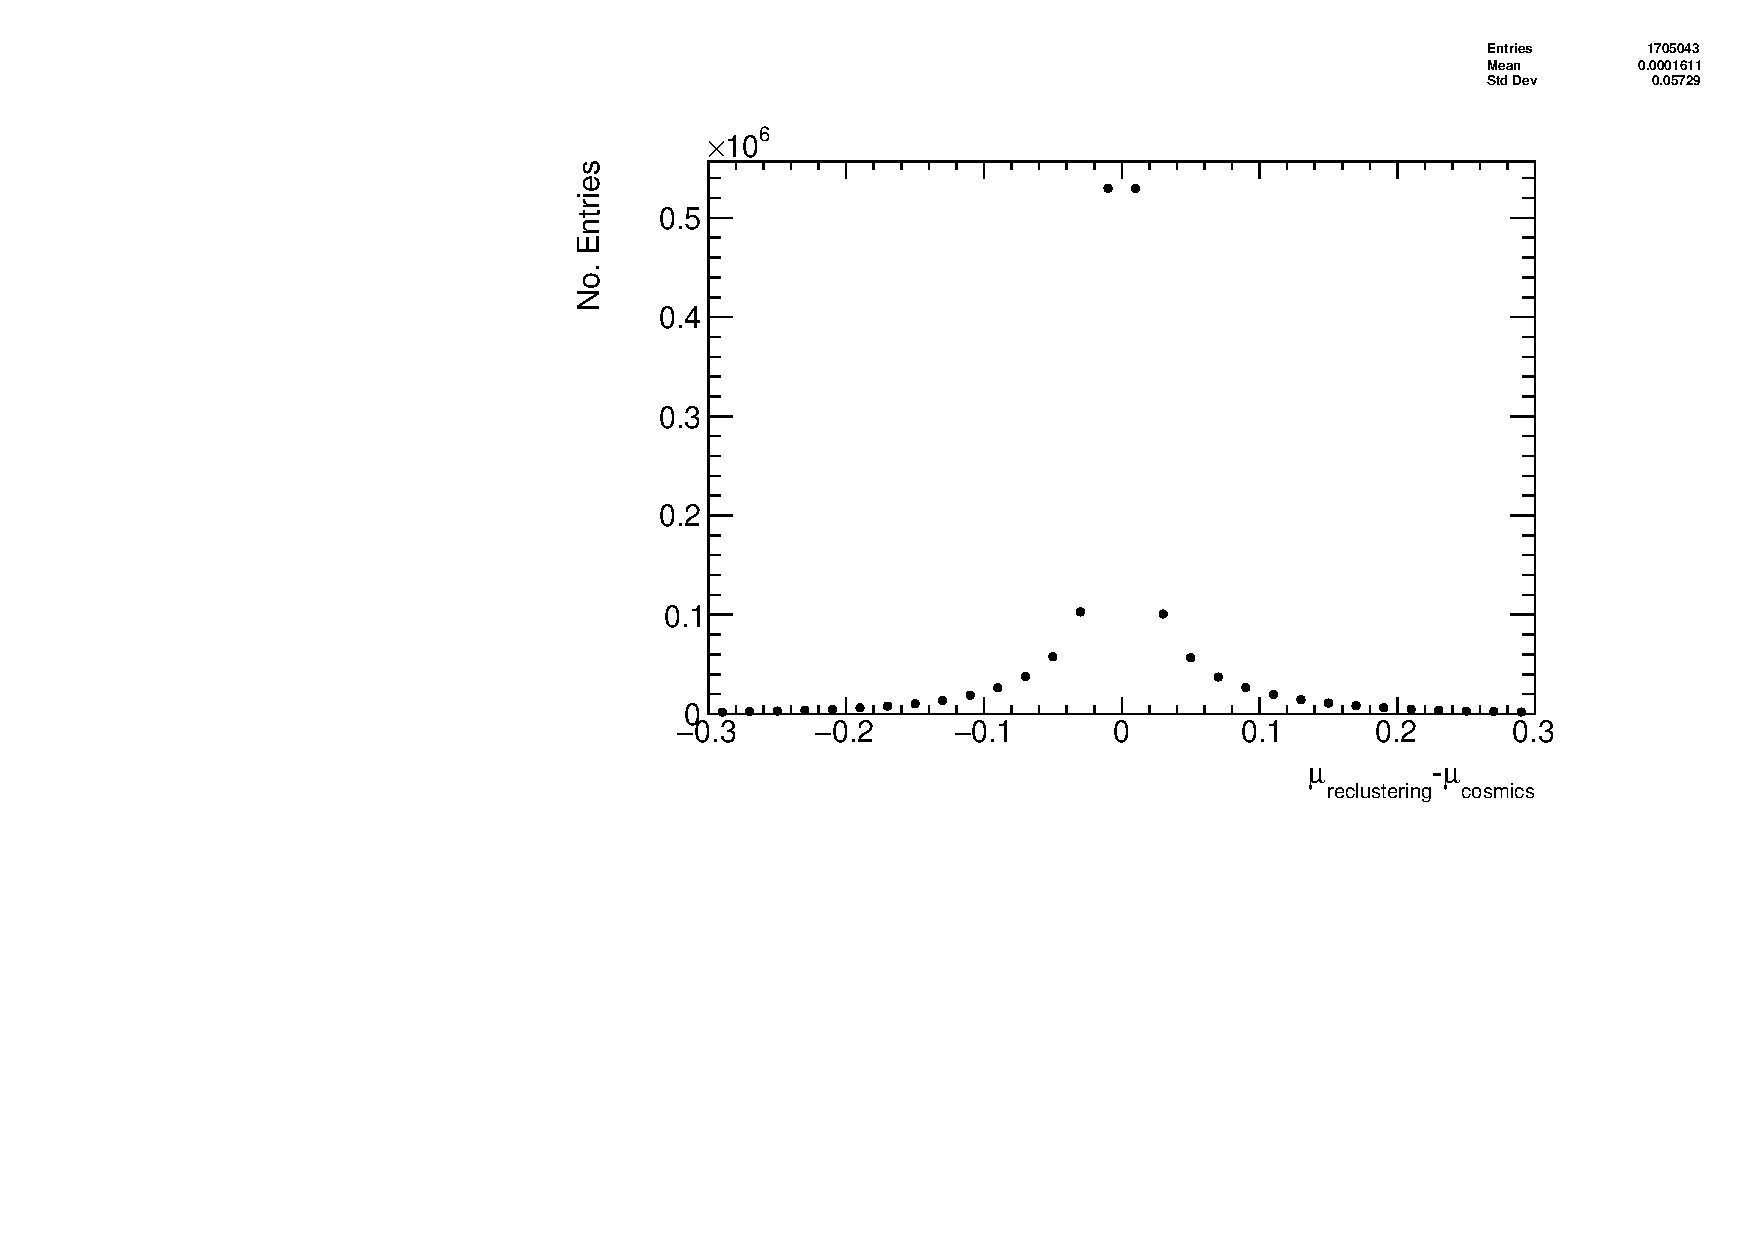
\includegraphics[width = 0.7\textwidth]{figures/figure_QL2P08_3100V_2021-05-21_reclustering_plots_mu_reclustering_minus_mu_cosmics.pdf}
    \caption{The difference between cluster means calculated with Guo's method~\cite{guo_simple_2011} in \package{tgc\_analysis/CosmicsAnalysis} and Minuit2 for ROOT~\cite{hatlo_developments_2005} in \package{strip\_position\_analysis/ReClustering} for data collected with QL2.P.8 at 3.1~kV.}
    \label{fig:mu_reclustering_minus_mu_cosmics}
\end{figure}

The RMS of the distribution in figure~\ref{fig:mu_reclustering_minus_mu_cosmics} is \SI{57}{\micro\meter}, which is much larger than the statistical uncertainty in the mean for the Minuit2 algorithm, which peaks around \SI{7}{\micro\meter}. An RMS of \SI{57}{\micro\meter} is common for data taken with most quadruplets at 3.1~kV. Therefore, the uncertainty in the y-hit positions is assigned \SI{57}{\micro\meter}.

The uncertainty assigned to the hit position affected the uncertainty in the extrapolated/interpolated position of the track, and in the residuals. The bin size of the residual distributions was \SI{200}{\micro\meter} because that was the uncertainty in the residuals calculated from the tracks with the least favourable geometry (like tracks built from hits on layers 1 and 2 and extrapolated to layer 4). 

The x position of the hit was taken to be the center of the wire group with the maximum peak detector output, since wire groups are much wider than the typical charge distribution spread. Assuming that the true x-position of the hit is uniformly distributed over the width of the wire group, the uncertainty in the x-position is given by $\frac{w}{\sqrt(12)}$, where $w$ is the width of the wire group~\cite{Sauli:117989}. sTGC wire groups are \SI{36}{\milli\meter} wide so the hit x-position uncertainty was $10 mm$.

%TODO : How does this inform the area of the bins we take residual means in?

%TODO : How does reclustering affect residual means?
